% https://es.overleaf.com/latex/templates/project-report/jpzczmpsdzwm

%%% Preamble
\documentclass[paper=leter, fontsize=11pt]{scrartcl}
\usepackage[utf8]{inputenc}
\usepackage[spanish,mexico]{babel}
\usepackage[T1]{fontenc}    % use 8-bit T1 fonts
\usepackage{lmodern}
\usepackage{hyperref}       % hyperlinks
\usepackage{lipsum}
\usepackage[square,numbers]{natbib}

\usepackage[protrusion=true,expansion=true]{microtype}	
\usepackage{amsmath,amsfonts,amsthm} % Math packages
\usepackage[pdftex]{graphicx}
\usepackage{url}

\usepackage{booktabs}

\usepackage{tikz}

\usepackage{caption}
\usepackage{subcaption}

\usepackage{listings}
\lstdefinestyle{mystyle}{
    basicstyle=\ttfamily\footnotesize,
    breakatwhitespace=false,         
    breaklines=true,                 
    captionpos=b,                    
    keepspaces=true,                 
    numbers=left,                    
    numbersep=5pt,                  
    showspaces=false,                
    showstringspaces=false,
    showtabs=false,                  
    tabsize=4
}

\lstset{style=mystyle}
\renewcommand{\lstlistingname}{Código}

\graphicspath{ {img/} }

\selectlanguage{spanish}
\usepackage[spanish,onelanguage,ruled]{algorithm2e}


%%% Custom sectioning
\usepackage{sectsty}
\allsectionsfont{\centering \normalfont\scshape}


%%% Custom headers/footers (fancyhdr package)
\usepackage{fancyhdr}
\pagestyle{fancyplain}
\fancyhead{}											% No page header
\fancyfoot[L]{}											% Empty 
\fancyfoot[C]{}											% Empty
\fancyfoot[R]{\thepage}									% Pagenumbering
\renewcommand{\headrulewidth}{0pt}			% Remove header underlines
\renewcommand{\footrulewidth}{0pt}				% Remove footer underlines
\setlength{\headheight}{13.6pt}


%%% Equation and float numbering
\numberwithin{equation}{section}		% Equationnumbering: section.eq#
\numberwithin{figure}{section}			% Figurenumbering: section.fig#
\numberwithin{table}{section}				% Tablenumbering: section.tab#


%%% Maketitle metadata
\newcommand{\horrule}[1]{\rule{\linewidth}{#1}} 	% Horizontal rule

%%% https://tex.stackexchange.com/a/118217
\usepackage{mathtools}
\DeclarePairedDelimiter\ceil{\lceil}{\rceil}
\DeclarePairedDelimiter\floor{\lfloor}{\rfloor}

\usepackage{amsmath}

\usepackage{tikz}

\title{
		%\vspace{-1in} 	
		\usefont{OT1}{bch}{b}{n}
		\normalfont \normalsize \textsc{Posgrado de Ingeniería de Sistemas} \\ [25pt]
		\horrule{0.5pt} \\[0.4cm]
		\huge Unir-encontrar \\
		\horrule{2pt} \\[0.5cm]
}
\author{
		\normalfont 								\normalsize
        Alberto Benavides\\[-3pt]		\normalsize
        \today
}
\date{}


%%% Begin document
\begin{document}
\maketitle

\section{Introducción}

Las operaciones de \textit{unir-encontrar} permiten realizar funciones de búsqueda y unión en conjuntos que tengan elementos con identificadores irrepetibles entre sí. Una manera de representar conjuntos y sus elementos es mediante grafos en que cada nodo corresponde a cada elemento, mientras que grafos disjuntos equivalen a conjuntos, lo cual aparece representado en los incisos de la figura \ref{tres_grafos}.


\begin{figure}
    \begin{subfigure}{.45\textwidth}
        \centering
        \begin{tikzpicture}
            \node[draw, circle] at (0, 0) {$e$};
        \end{tikzpicture}
        \caption{Un conjunto $C = \{e\}$ representado por un nodo}
        \label{nodo}
    \end{subfigure}
    \hfill
    \begin{subfigure}{.45\textwidth}
        \centering
        \begin{tikzpicture}
            \node[draw, circle] (e1) at (0, 0) {$e_1$};
            \node[draw, circle] (e2) at (2, 0) {$e_2$};
            \node[draw, circle] (e3) at (4, 0) {$e_3$};
            
            \draw[] (e1) -- (e2);
            \draw[] (e2) -- (e3);
        \end{tikzpicture}
        \caption{Un conjunto \(C = \{e_1, e_2, e_3\}\) representado por un grafo con tres nodos.}
        \label{grafo}
    \end{subfigure}

    \vspace{1cm}
    
    \centering
    \begin{subfigure}{0.45\textwidth}
        \centering
        \begin{tikzpicture}
            \node[draw, circle] (e1) at (0, 0) {$e_1$};
            \node[draw, circle] (e2) at (2, 0) {$e_2$};
            \node[draw, circle] (e3) at (4, 0) {$e_3$};
            
            \draw[] (e2) -- (e3);
        \end{tikzpicture}
        \caption{Los conjuntos \(C_1 = \{e_1\}\) y \(C_2 = \{e_2, e_3\}\) representados por dos grafo.}
        \label{grafos}
    \end{subfigure}

    \caption{Ejemplos de representación de conjuntos y elementos por grafos.}
    \label{tres_grafos}
\end{figure}

En este caso, la unión de dos conjuntos se realiza mediante la función de búsqueda primeramente. Esta última función consiste en devolver todos los elementos pertenecientes a un conjunto. Una manera de implementar esto es construir un diccionario en el que a cada elemento se le asigne un índice $i = \{0, 1, 2, \ldots\}$ y se asocie con el índice $p$ un nodo de otro grafo al que se haya unido. A este otro nodo se le denomina \textit{padre}, por comodidad. Cuando un elemento se tiene por padre a sí mismo se considera que forma parte de un conjunto con un solo elemento. Esto se ejemplifica en la tabla \ref{asignacion}.

\begin{table}[]
    \centering
    \caption{Ejemplo de asignación de índices a elementos de un conjunto.}
    \label{asignacion}
    \begin{tabular}{@{}ccccc@{}}
    \toprule
    Elemento & $e_1$ & $e_1$ & $e_1$ & $\ldots$ \\ \midrule
    Padre   & $0$     & $1$     & $2$     & $\ldots$ \\ \bottomrule
    Índice   & $0$     & $1$     & $2$     & $\ldots$ \\ \bottomrule
    \end{tabular}
\end{table}

Unir dos conjuntos a partir de los elementos $e_1 \in C_1$ y $e_2 \in C_2$ consiste en definir qué nodo será padre del otro, aquí $e_1$ será padre de $e_2$. Luego, se recorren todos los padres del nodo hijo hasta encontrar uno que no tenga ningún padre, lo que puede hacerse en tiempo $\mathcal{O}(n)$. Una vez encontrado el nodo que no tiene padre, se le asigna como padre a $e_1$ y esto resulta en la unión de dos conjuntos representados por grafos con nodos. Una ilustración al respecto puede consutarse en la imagen \ref{ejemplo_union}.

\begin{figure}
    \begin{subfigure}{.45\textwidth}
        \centering
        \begin{tikzpicture}
            \node[draw, circle] (e1) at (0, 0) {$e_1$};
            \node[draw, circle] (e2) at (2, 0) {$e_2$};
            \node[draw, circle] (e3) at (4, 0) {$e_3$};
            
            \draw[->] (e2) -- (e3);
        \end{tikzpicture}
        \caption{Se desea unir $C_1 = \{e_1\}$ con $C_2 = \{e_2, e_3\}$ a partir de $e_1$ y $e_3$.}
        \label{nodo}
    \end{subfigure}
    \hfill
    \begin{subfigure}{.45\textwidth}
        \centering
        \begin{tikzpicture}
            \node[draw, circle] (e1) at (0, 0) {$e_1$};
            \node[draw, circle] (e2) at (2, 0) {$e_2$};
            \node[draw, circle] (e3) at (4, 0) {$e_3$};
            
            \draw[->] (e1) -- (e2);
            \draw[->] (e2) -- (e3);
        \end{tikzpicture}
        \caption{Como $e_3$ tiene por padre a $e_2$ quien no tiene padre, se le asigna $e_1$ como padre a $e_2$.}
        \label{grafo}
    \end{subfigure}

    \caption{Ejemplo de unión de un conjunto $C_1 = \{e_1\}$ con un conjunto $C_2 = \{e_2, e_3\}$.}
    \label{ejemplo_union}
\end{figure}

Una implementación interactiva de esto puede consultarse en \url{https://jbenavidesv87.github.io/algoritmos/union-find.html}. La implementación funciona a partir de tres métodos de entrada (véase la figura \ref{pantalla_inicio}). El primero permite crear conjuntos con un elemento único, representados por nodos disjuntos. Los otros dos métodos de entrada permiten especificar el valor del elemento del primer conjunto que desea unirse con el valor del elemento de un segundo conjunto.

\begin{figure}
    \centering
    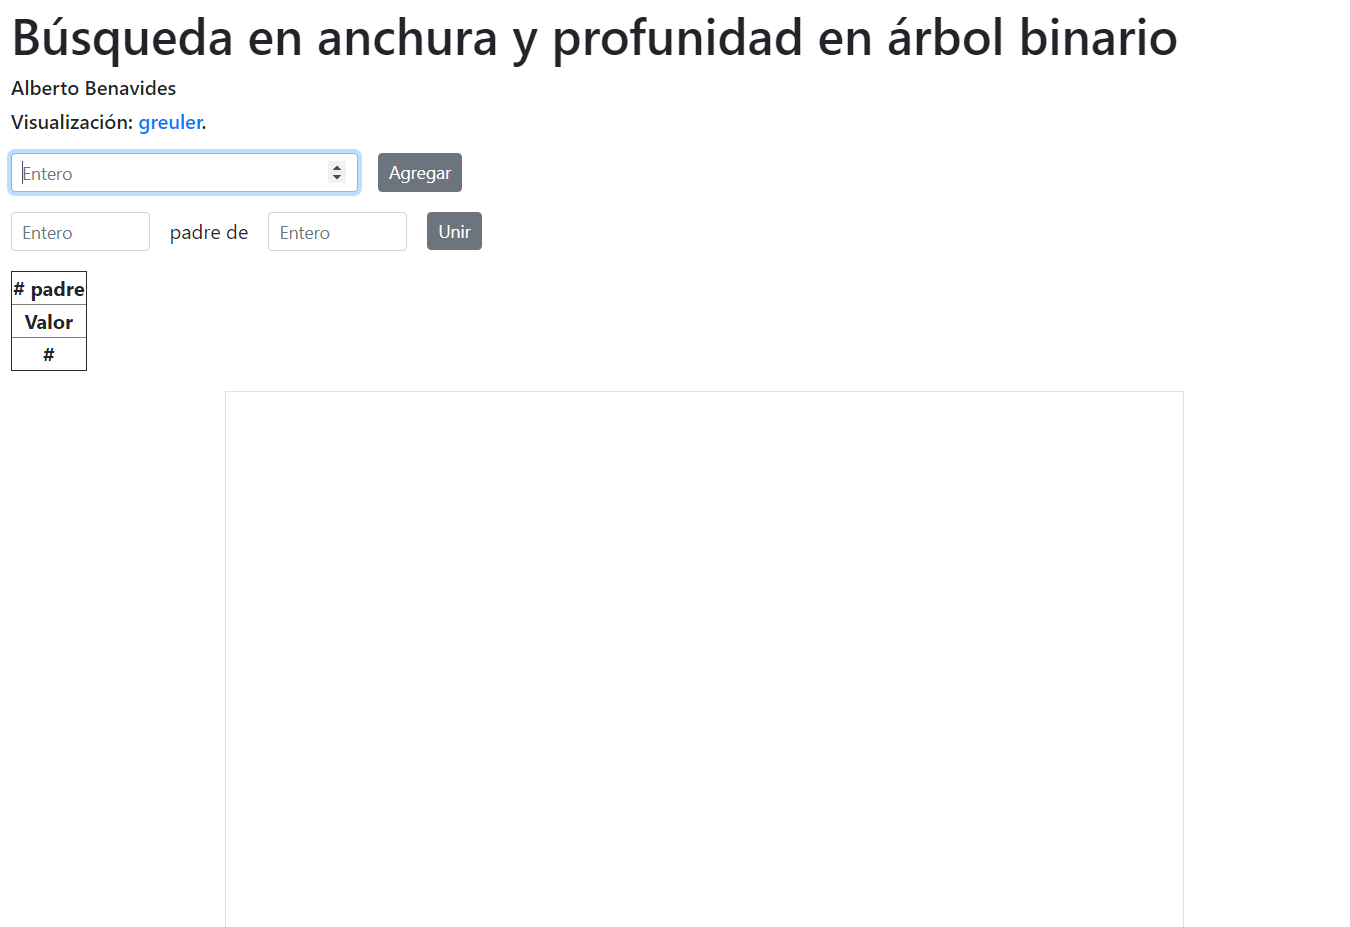
\includegraphics[width=0.8\textwidth]{1.png}
    \caption{Pantalla inicial del interactivo desarrollado.}
    \label{pantalla_inicio}
\end{figure}

Las figuras \ref{agregado_nodos, union_uno, union_dos} muestran, en ese orden, el ejemplo de agregado de nodos, unión entre nodos disjuntos y unión de dos conjuntos disjuntos a partir de dos de sus elementos.

\begin{figure}
    \centering
    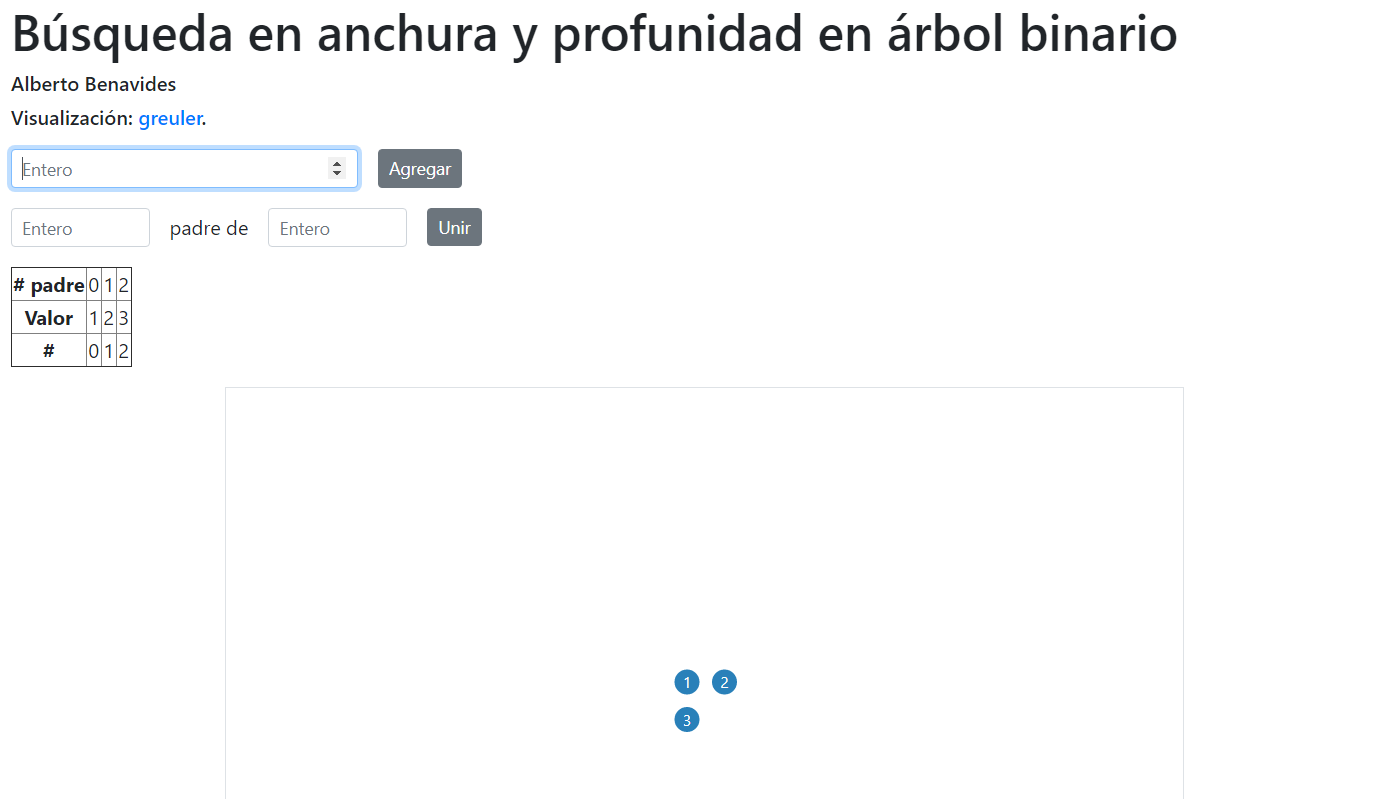
\includegraphics[width=0.8\textwidth]{2.png}
    \caption{Ejemplo de agregado de tres elementos con valores $1, 2, 3, 4$.}
    \label{agregado_nodos}
\end{figure}

\begin{figure}
    \centering
    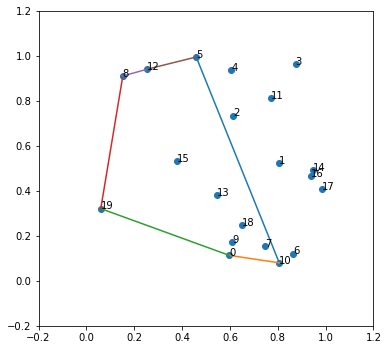
\includegraphics[width=0.8\textwidth]{5.png}
    \caption{Unión del nodo $1$ con el $2$ y el $3$ con el $4$.}
    \label{union_uno}
\end{figure}

\begin{figure}
    \centering
    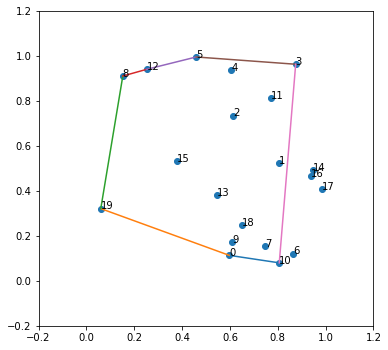
\includegraphics[width=0.8\textwidth]{6.png}
    \caption{Ejemplo de unión del nodo $3$ con el $1$.}
    \label{union_dos}
\end{figure}

\bibliographystyle{plainnat}
\bibliography{Biblio}

\end{document}